\documentclass[aspectratio=169]{beamer}

% Suppress all navigation symbols
\setbeamertemplate{navigation symbols}{}
\setbeamertemplate{headline}{}
\setbeamertemplate{footline}{}
\setbeamertemplate{itemize items}[circle]
\setbeamertemplate{footline}[frame number]

\setbeamercolor{structure}{fg=blue}
\setbeamercolor{normal text}{fg=black, bg=white}
\setbeamerfont{title}{series=\bfseries, size=\Huge}
\setbeamerfont{frametitle}{series=\bfseries, size=\LARGE}

\setbeamertemplate{footline}{
  \begin{tikzpicture}[remember picture,
                      overlay,
                      shift={(current page.south west)}]
    \node [black!50, inner sep=2mm, anchor=south east]
          at (current page.south east)
          {\large \bfseries \insertframenumber};
  \end{tikzpicture}
}

\definecolor{red}{RGB}{220, 50, 47}
\definecolor{green}{RGB}{133, 153, 0}
\definecolor{cyan}{RGB}{42, 161, 152}
\definecolor{blue}{RGB}{38, 139, 210}
\definecolor{yellow}{RGB}{181, 137, 0}

\usepackage{fontspec}
\setsansfont{Overpass}[Scale=MatchLowercase]
\setmonofont{Overpass Mono}[Scale=MatchLowercase]

\usepackage{listings}
\lstset{
  basicstyle=\ttfamily\small,
  commentstyle={\color{black!50}},
  language=Java,
}

\usepackage{pgfplots}

\usepackage{tikz}
\usetikzlibrary{arrows}
\usetikzlibrary{backgrounds}
\usetikzlibrary{calc}
\usetikzlibrary{decorations.pathreplacing}
\usetikzlibrary{fit}
\usetikzlibrary{positioning}
\usetikzlibrary{matrix}
\usetikzlibrary{scopes}
\usetikzlibrary{shapes}
\usetikzlibrary{tikzmark}
\usetikzmarklibrary{listings}

\tikzset{
    arrow/.style={->,>=stealth', shorten >=2pt, thick},
    box/.style = {
      minimum size=0.6cm,
      rounded corners,
      rectangle,
      fill=blue!50
    },
    bigbox/.style = {
      draw=blue!50,
      thick,
      fill=blue!10,
      rounded corners,
      rectangle
    },
}


\title{JDebloat: Overview}
\author{Jon Eyolfson}
\date{2020-02-26}

\setbeamertemplate{title page}
{
  \begin{tikzpicture}[remember picture,
                      overlay,
                      shift={(current page.south west)}]
    \node (title) [inner sep=0, scale=1.2, align=center]
          at (\paperwidth / 2, \paperheight * 2 / 3)
          {\usebeamerfont{title}\usebeamercolor[fg]{title} \inserttitle};
    \node (author) [scale=1.5] at (\paperwidth / 2, \paperheight / 3)
          {\insertauthor};
    \node [anchor=south east, inner sep=2mm] at (\paperwidth, 0)
          {\bfseries \insertdate};
  \end{tikzpicture}
}

\begin{document}

  \begin{frame}[plain]
    \titlepage
  \end{frame}

  \setcounter{framenumber}{0}

  \begin{frame}
    \frametitle{Push-Button Debloating}

    \begin{center}
      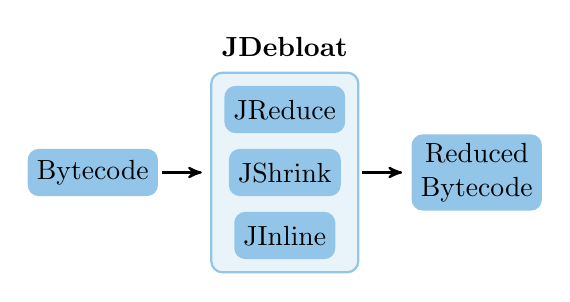
\begin{tikzpicture}[
        outer sep=0.05cm,
        node distance=0.8cm
      ]
        \tikzstyle{bigbox} = [
          draw=blue!50,
          thick,
          fill=blue!10,
          rounded corners,
          rectangle
        ]
        \tikzstyle{box} = [
          minimum size=0.6cm,
          rounded corners,
          rectangle,
          fill=blue!50
        ]

        \node[box] (1) {JReduce};
        \node[box,below of=1] (2) {JShrink};
        \node[box,below of=2] (3) {JInline};

        \begin{pgfonlayer}{background}
          \node[bigbox] [fit = (1) (3)] (jdebloatbox) {};
        \end{pgfonlayer}

        \node[box, left=of 2.west, anchor=east] (input) {Bytecode};
        \node[box, right=of 2.east, anchor=west, align=center] (output) {Reduced\\Bytecode};

        \draw[arrow] (input.east) -- (jdebloatbox);
        \draw[arrow] (jdebloatbox.east) -- (output.west);

        \node [above of=1] {\bfseries JDebloat};
      \end{tikzpicture}
    \end{center}

    \vspace{2em}

    Just run \texttt{./jdebloat} on a JAR file (with tests)
  \end{frame}

  \begin{frame}
    \frametitle{We Added More Extensive Benchmarks}

    \begin{center}
      \LARGE 7 $\to$ \textbf{25}
    \end{center}

    \vspace{4em}

    Largest program has 175,548 methods (previous largest 3,586)
  \end{frame}

  \begin{frame}
    \frametitle{JReduce: A Dynamic Java Bytecode Reducer}

    Focus on buggy input reduction to decompilers, instead of tree-shaking

    \vspace{4em}

    Extended idea to remove methods and fields (instead of classes)
  \end{frame}

  \begin{frame}
    \frametitle{JReduce Uses Tests to Remove Code}
    \centering
    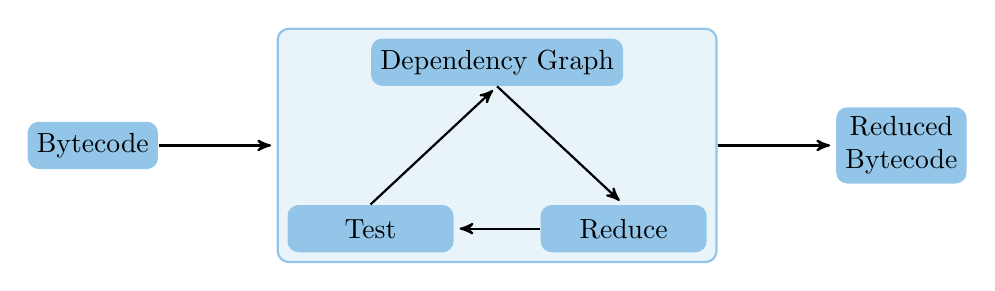
\begin{tikzpicture}
      \node [box] (dependencygraph) {Dependency Graph};

      \node [
        box,
        minimum width=6em,
        below=1.5cm and .75cm of dependencygraph.south west,
      ] (test) {Test};

      \node [
        box,
        minimum width=6em,
        below=1.5cm and .75cm of dependencygraph.south east,
      ] (reduce) {Reduce};

      \draw[arrow] (dependencygraph.south) -- (reduce.north);
      \draw[arrow] (reduce.west) -- (test.east);
      \draw[arrow] (test.north) -- (dependencygraph.south);

      \begin{pgfonlayer}{background}
        \node[draw, bigbox,fit=(dependencygraph) (test) (reduce)] (outline) {};
      \end{pgfonlayer}

      \node [box, left=1.5cm of outline] (input) {Bytecode};
      \node [box, right=1.5cm of outline, align=center] (output) {Reduced\\Bytecode};

      \draw[arrow] (input.east) -- (outline.west);
      \draw[arrow] (outline.east) -- (output.west);
    \end{tikzpicture}
  \end{frame}

  \begin{frame}
    \frametitle{JReduce Produced Better Reduction}

    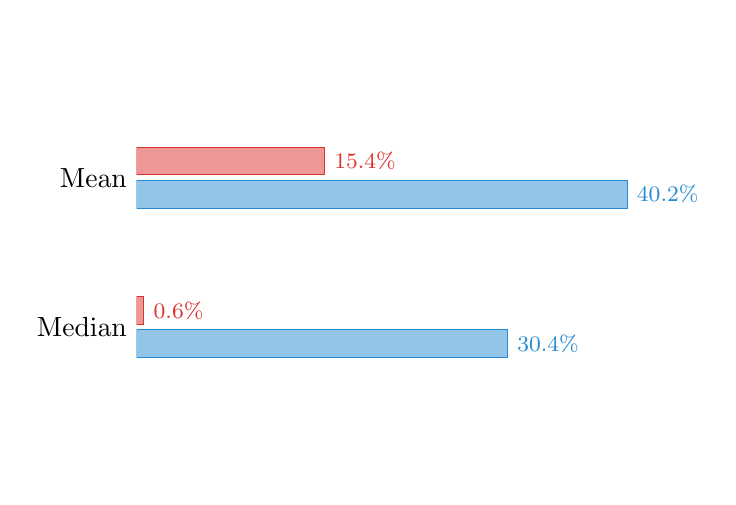
\begin{tikzpicture}
      \begin{axis}[
        xbar,
        y axis line style = {opacity = 0},
        axis x line       = none,
        xmin = 0,
        tickwidth         = 0pt,
        enlarge y limits  = 1,
        symbolic y coords = {Median,Mean},
        ytick             = data,
        nodes near coords,
        nodes near coords style={font=\footnotesize},
        nodes near coords align={anchor=west},
        point meta=explicit symbolic,
      ]
        \addplot [color=blue,fill=blue!50] coordinates {
          (40.2,Mean) [40.2\%]
          (30.4,Median) [30.4\%]
        };
        \addplot [color=red, fill=red!50]  coordinates {
          (15.4,Mean) [15.4\%]
          (0.6,Median) [0.6\%]
        };
      \end{axis}
    \end{tikzpicture}

    \vspace{-2em}

    Magnitude faster results compared to delta-debugging

    \vspace{2em}

    \textbf{Published in [FSE'19]}
  \end{frame}

  \begin{frame}
    \frametitle{JReduce Is Improving its Modeling Language}


    Switching from Graphics to Logics

    \vspace{2em}

    8.1 times better reduction than \textbf{[FSE'19]}, while only being 0.57
    times slower
  \end{frame}

  \begin{frame}
    \frametitle{JShrink Removes Unused Code Through Analysis}

    JShrink performs 4 transformations:
    \begin{enumerate}
      \item Unused method removal
      \item Unused field removal
      \item Static inlining
      \item Class collapsing / class hierarchy specialization
    \end{enumerate}

    \vspace{2em}

    Builds a static call graph, and handles reflection by adding dynamic
    information

    \vspace{2em}

    Able to specify program entry points
  \end{frame}

  \begin{frame}
    \frametitle{JShrink Uses Call Graph Analysis to Reduce Code Size}

    \centering
    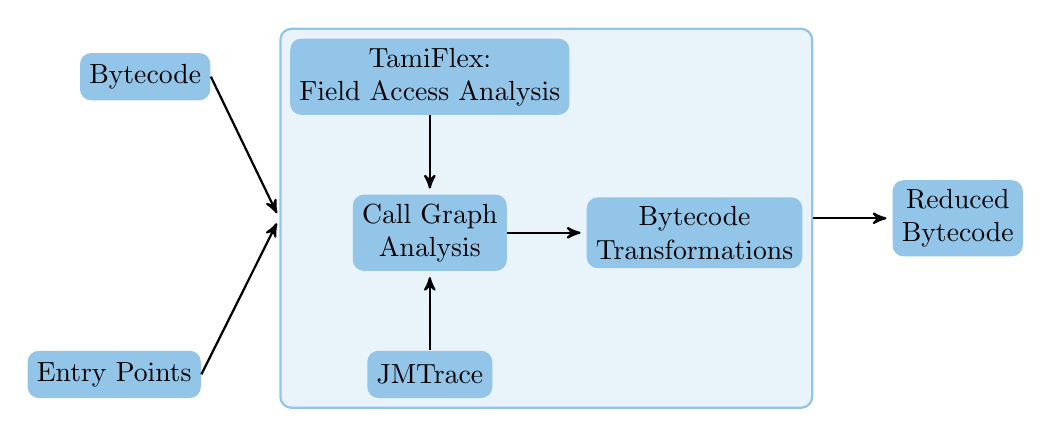
\begin{tikzpicture}
      \node[box, align=center] (cga) {Call Graph\\Analysis};
      \node[box, right=of cga, align=center] (bytecodetransformations) {Bytecode\\Transformations};
      \node[box, above=of cga, align=center] (tamiflex) {TamiFlex:\\Field Access Analysis};
      \node[box, below=of cga] (jmtrace) {JMTrace};

      \draw[arrow] (tamiflex) -- (cga.north);
      \draw[arrow] (cga) -- (bytecodetransformations);
      \draw[arrow] (jmtrace) -- (cga.south);

      \begin{pgfonlayer}{background}
        \node[draw, bigbox, fit=(cga) (bytecodetransformations) (tamiflex) (jmtrace)] (jshrink) {};
      \end{pgfonlayer}

      \node[box, left=of tamiflex] (inputbc) {Bytecode};
      \node[box, left=2.1cm of jmtrace, align=center] (entrypoints) {Entry Points};

      \node[box, right=of jshrink, align=center] (output) {Reduced\\Bytecode};

      \draw[arrow] (jshrink.east) -- (output.west);
      \draw[arrow] (inputbc.east) -- (jshrink.west);
      \draw[arrow] (entrypoints.east) -- (jshrink.west);
    \end{tikzpicture}
  \end{frame}

  \begin{frame}
    \frametitle{JShrink Handles More Dynamic Features}

    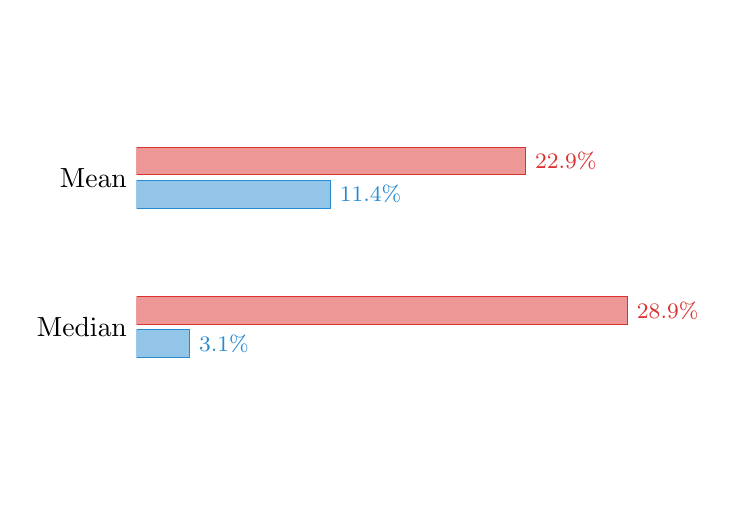
\begin{tikzpicture}
      \begin{axis}[
        xbar,
        y axis line style = {opacity = 0},
        axis x line       = none,
        xmin = 0,
        tickwidth         = 0pt,
        enlarge y limits  = 1,
        symbolic y coords = {Median,Mean},
        ytick             = data,
        nodes near coords,
        nodes near coords style={font=\footnotesize},
        nodes near coords align={anchor=west},
        point meta=explicit symbolic,
      ]
        \addplot [color=blue,fill=blue!50] coordinates {
          (11.4,Mean) [11.4\%]
          (3.1,Median) [3.1\%]
        };
        \addplot [color=red, fill=red!50]  coordinates {
          (22.9,Mean) [22.9\%]
          (28.9,Median) [28.9\%]
        };
      \end{axis}
    \end{tikzpicture}

    \vspace{-2em}

    We developed a profiling tool named JMTrace for our dynamic analysis
    (submitted to \textbf{[FSE'20]})
  \end{frame}

  \begin{frame}
    \frametitle{JShrink May Help Developers}

    Extensive comparison with ProGuard

    \vspace{2em}

    Includes rollback feature to ensure semantic preservation
  \end{frame}

  \begin{frame}[fragile]
    \frametitle{JInline Finds Call Sites to Inline}

    We replace a method call with the method body

    \vspace{2em}

    Allows us to remove the method (and maybe even library)

  \end{frame}

  \begin{frame}[fragile]
    \frametitle{JInline Uses Program Behavior to Inline Code}

    \centering
    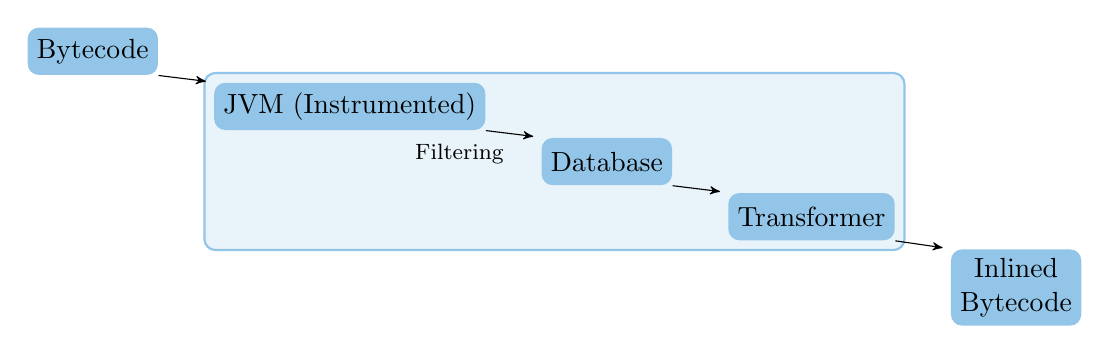
\begin{tikzpicture}[
      node distance=0.7cm, ->, >=stealth', shorten >=1mm
    ]
      \node [box] (original) {Bytecode};
      \node [box, right=of original, yshift=-0.7cm] (jvm) {JVM (Instrumented)};
      \node [box, right=of jvm, yshift=-0.7cm] (database) {Database};
      \node [box, right=of database, yshift=-0.7cm] (jinliner)
            {Transformer};
      \node [box, right=of jinliner, yshift=-0.9cm, align=center] (modified) {Inlined\\Bytecode};

      \begin{pgfonlayer}{background}
        \node[draw, bigbox, fit=(jvm) (database) (jinliner)] (jinline) {};
      \end{pgfonlayer}

      \path (original.south east) edge (jvm.north west)
            (jvm.south east) edge
              node [below left] {\footnotesize Filtering} (database.north west)
            (database.south east) edge (jinliner.north west)
            (jinliner.south east) edge (modified.north west);
    \end{tikzpicture}

  \end{frame}

  \begin{frame}
    \frametitle{JInline Is More Aggressive}

    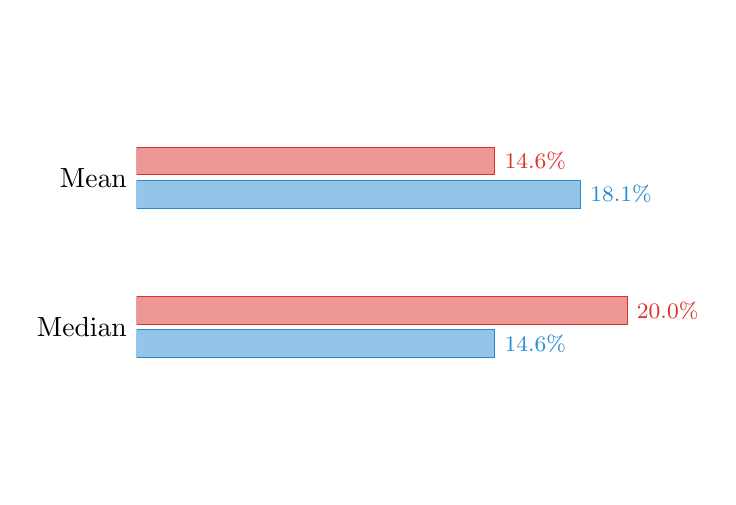
\begin{tikzpicture}
      \begin{axis}[
        xbar,
        y axis line style = {opacity = 0},
        axis x line       = none,
        xmin = 0,
        tickwidth         = 0pt,
        enlarge y limits  = 1,
        symbolic y coords = {Median,Mean},
        ytick             = data,
        nodes near coords,
        nodes near coords style={font=\footnotesize},
        nodes near coords align={anchor=west},
        point meta=explicit symbolic,
      ]
        \addplot [color=blue,fill=blue!50] coordinates {
          (18.1,Mean) [18.1\%]
          (14.6,Median) [14.6\%]
        };
        \addplot [color=red, fill=red!50]  coordinates {
          (14.6,Mean) [14.6\%]
          (20.0,Median) [20.0\%]
        };
      \end{axis}
    \end{tikzpicture}

    \vspace{-2em}

    Inlines targets that don't have a single receiver

    \vspace{2em}

    \textbf{[SOSP'19]} submission related to reducing library dependence
  \end{frame}

  \begin{frame}
    \frametitle{JInline Further Increases its Reach}

    Currently inlines all targets

    \vspace{2em}

    In the future we want to inline call sites with many receivers, only if it
    helps other tools
  \end{frame}

  \begin{frame}
    \frametitle{All Tools Synergize Better Together}

    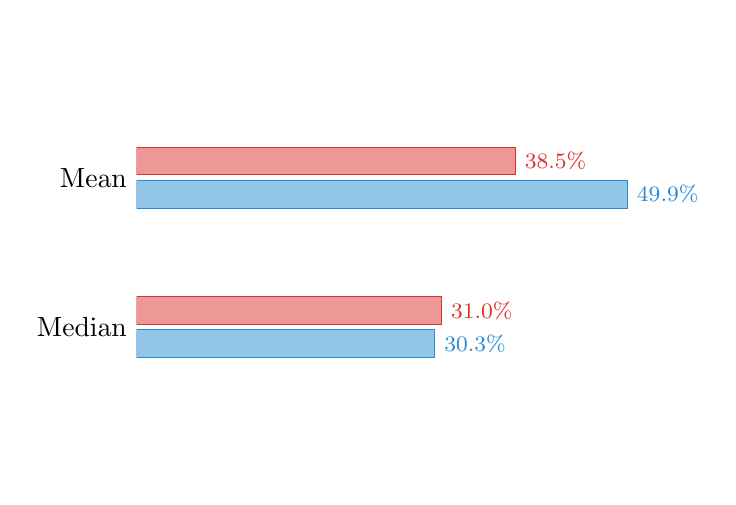
\begin{tikzpicture}
      \begin{axis}[
        xbar,
        y axis line style = {opacity = 0},
        axis x line       = none,
        xmin = 0,
        tickwidth         = 0pt,
        enlarge y limits  = 1,
        symbolic y coords = {Median,Mean},
        ytick             = data,
        nodes near coords,
        nodes near coords style={font=\footnotesize},
        nodes near coords align={anchor=west},
        point meta=explicit symbolic,
      ]
        \addplot [color=blue,fill=blue!50] coordinates {
          (49.9,Mean) [49.9\%]
          (30.3,Median) [30.3\%]
        };
        \addplot [color=red, fill=red!50]  coordinates {
          (38.5,Mean) [38.5\%]
          (31.0,Median) [31.0\%]
        };
      \end{axis}
    \end{tikzpicture}

    \vspace{-2em}

    Recall, our benchmarks are orders of magnitude larger
  \end{frame}

\end{document}
